\documentclass[12pt,a4paper]{article}
\usepackage[utf8x]{inputenc}
\usepackage{ucs}
\usepackage[english,russian]{babel}
\usepackage[OT1]{fontenc}
\usepackage{amsmath}
\usepackage{amsfonts}
\usepackage{amssymb}
\usepackage{wasysym}
\usepackage{physics}
\usepackage{wrapfig}
\usepackage{mathrsfs}

%---------Схемы---------
\usepackage{circuitikz}
%-----------------------

%--------Графики--------
\usepackage{pgfplots}
%Чтобы хорошо работало
\pgfplotsset{compat=1.9}
%----------------------

\usepackage[left=2cm,right=2cm,top=2cm,bottom=2cm,includefoot,footskip=1.5cm]{geometry}

\usepackage{fancyhdr}
\pagestyle{fancy}

\usepackage[T1]{fontenc}
 
\usepackage{indentfirst}
%% Sets page size and margins
%\usepackage[dvips]{graphicx}
%\graphicspath{{noiseimages/}}
%\usepackage[colorinlistoftodos]{todonotes}
%\usepackage[colorlinks=true, allcolors=blue]{hyperref}

\rhead{\small Д.\,Павлов, МФТИ}
\lhead{Лабораторная работа №3.4.2}

\author{Дмитрий Павлов, 790}
\title {\textbf{Закон Кюри-Вейсса.}}

\begin{document}
\maketitle
\newpage
\tableofcontents 

\newpage

\section{Вступление.}
    \subsection{Цель работы.}
        Определить парамагнитную точку Кюри гадолиния по зависимости периода колебаний автогенератора от температуры сердечника катушки.
        
    \subsection{Оборудование.}
        \begin{itemize}
            \item Катушка самоиндукции с образцом из гадолиния;
            \item Термостат;
            \item Частотомер;
            \item Цифровой вольтметр;
            \item LC-автогенератор;
            \item Термопара медь-константан.
        \end{itemize}

    \subsection{Экспериментальная установка.}
        \begin{center}
            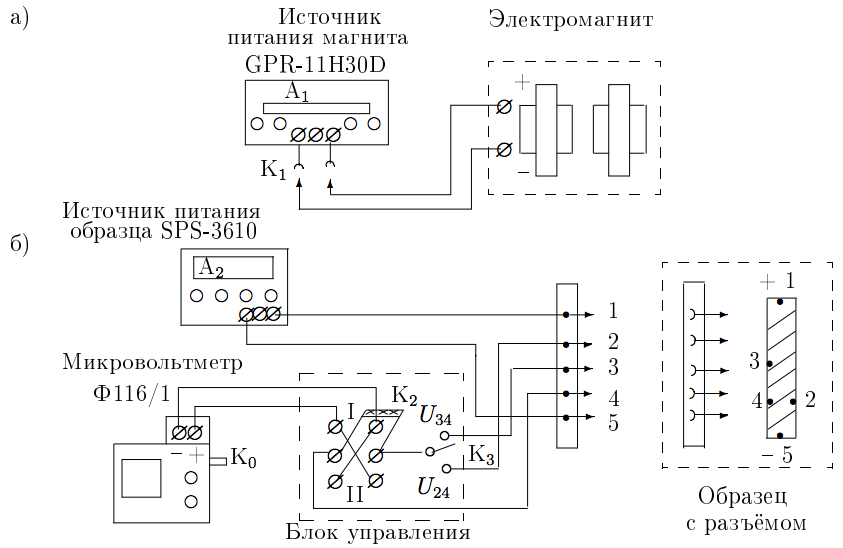
\includegraphics[width=0.8\linewidth]{img/img1.png}
            
            Схема экспериментальной установки.
         \end{center}
         
        Исследуемый ферромагнитный образец (гадолиний) расположен внутри пустотелой катушки самоиндукции. При изменении температуры меняется магнитная восприимчивость образца $\chi$, а следовательно, самоиндукция катушки и период колебаний $\tau$ автогенератора. Для измерения периода используется частотомер.
        
        Закон Кюри-Вейса справедлив, если выполнено соотношение
        \begin{equation}
            \dfrac{1}{\chi} \sim \big(T - \Theta_p\big) \sim \dfrac{1}{\tau^2-\tau_o^2},
        \end{equation}
        где $\tau_o$ - период колебаний в отсутствие образца.

        Разность температур воды и образца контролируется с помощью медно-константановой термопары 6 и цифрового вольтметра. Чувствительность термопары $k = 24 \text{ град/мВ}$.
        
\section{Словарь.}
    \begin{itemize}
        \item Закон Кюри — Вейса --- закон, описывающий магнитную восприимчивость ферромагнетика в области температур выше точки Кюри (то есть в парамагнитной области). 
     
        \item Ферромагнетик —-- вещество, которое (при температуре ниже точки Кюри) способно обладать намагниченностью в отсутствии внешнего магнитного поля и имеющее положительную магнитную восприимчивость, значительно большую единицы.
        
        \item Парамагнетик --— вещество, которое намагничивается во внешнем магнитном поле в направлении внешнего магнитного поля и имеющее положительную магнитную восприимчивость, значительно меньшую единицы. 
        \item Магнитная восприимчивость — физическая величина, характеризующая связь между магнитным моментом (намагниченностью) вещества и магнитным полем в этом веществе.
        \[
        \chi = \dfrac{J}{H},
        \]
        где $J$ --- намагниченность вещества под действием магнитного поля, \\ 
        $H$ --- напряженность магнитного поля.
    \end{itemize}
\newpage
\section{Измерения.}
    \subsection{Зависимость периода колебаний LC-генератора от температуры образца.}
        Исследуем зависимость периода колебаний LC-генератора от температуры образца, отмечая период колебаний $\tau$ по частотомеру, а температуру $T$ --- по показаниям дисплея термостата и цифровому вольтметру ($\Delta U$ с учетом знака).
        
        Проведем измерения в диапазоне от $14 \textdegree C$ до $40 \textdegree C$ через $2 \textdegree C$.
        
        \begin{table}[!h]
            \begin{flushleft}%\hspace{80}
           		\textbf{Таблица 1} -- Зависимость периода колебаний LC-генератора от температуры образца. $T$ --- температура термостата.\\
            \end{flushleft}
            \begin{center}
                \begin{tabular}{ | l | l | l | l | l | l | l | l |}
                    \hline
                    $T$, \textdegree C    &   14.4    &   16.12   &   18.09   &   20      &   22.02   &   24.02   &   26      \\
                    \hline
                    $B$, мТл    &   10.77   &   10.66   &   10.49   &   10.31   &   9.96    &   9.59    &   9.43    \\
                    \hline
                    $U$, мВ     &   -0.0035 & -0.0033   & -0.0056   & -0.0141   & -0.013    & -0.014    & -0.016    \\
                    \hline
                    $T$, \textdegree C    &   28.6    &   30.01   &   32      &   34      &   36      &   38      &   40      \\
                    \hline
                    $B$, мТл    &   9.33    &   9.28    &   9.25    &   9.22    &   9.20    & 9.19      & 9.17      \\
                    \hline
                    $U$, мВ     &   -0.014  &   -0.015  &   -0.016  &   -0.018  &   -0.018  & -0.018    & -0.017    \\
                    \hline
                \end{tabular}
            \end{center}
        \end{table}
    
        Период колебаний $\tau_0$ без образца: $\tau_0 = 9.045 \text{ мкс}$.
        
\section{Обработка результатов.}
    \subsection{Температура образца.}
        Рассчитаем температуру $T$ образца с учетом показаний термопары.
        \begin{table}[!h]
            \begin{flushleft}%\hspace{80}
           		\textbf{Таблица 2} -- Зависимость периода колебаний LC-генератора от температуры образца. $T'$ --- температура образца.\\
            \end{flushleft}
            \begin{center}
                \begin{tabular}{ | l | l | l | l | l | l | l | l |}
                    \hline
                    $T'$, \textdegree C  &   14.32   &   16.04   &   17.96   &   19.66   &   21.71   &   23.68   &   25.62   \\
                    \hline
                    $B$, мТл    &   10.77   &   10.66   &   10.49   &   10.31   &   9.96    &   9.59    &   9.43    \\
                    \hline
                    $U$, мВ     &   -0.0035 & -0.0033   & -0.0056   & -0.0141   & -0.013    & -0.014    & -0.016    \\
                    \hline
                    $T'$, \textdegree C  &   28.26   &   29.65   &   31.62  &   33.57  &   35.57  &   37.57  &  39.59    \\
                    \hline
                    $B$, мТл    &   9.33    &   9.28    &   9.25    &   9.22    &   9.20    & 9.19      & 9.17      \\
                    \hline
                    $U$, мВ     &   -0.014  &   -0.015  &   -0.016  &   -0.018  &   -0.018  & -0.018    & -0.017    \\
                    \hline
                \end{tabular}
            \end{center}
        \end{table}
    \subsection{График.}
        \begin{center}
            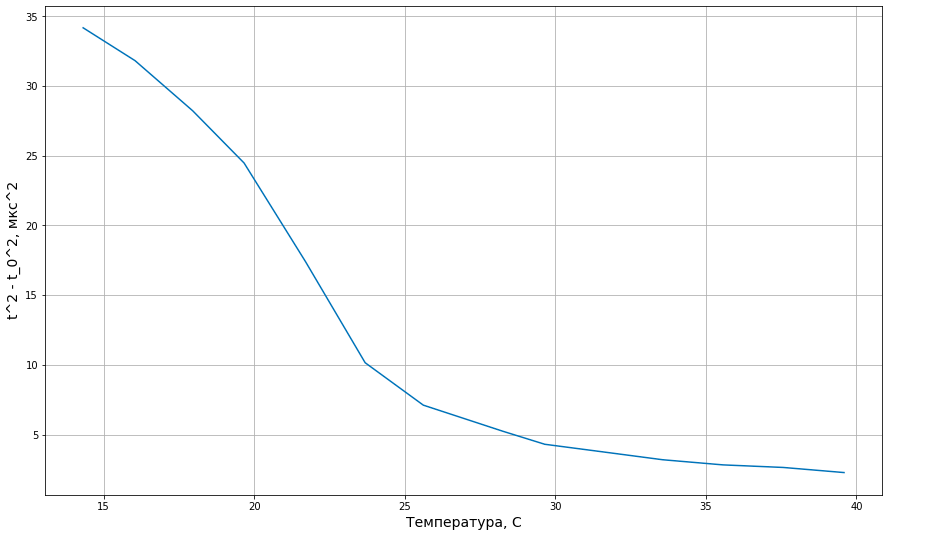
\includegraphics[width=0.9\linewidth]{img/img2.png}
            
            Определение температуры Кюри.
        \end{center}
        \begin{center}
            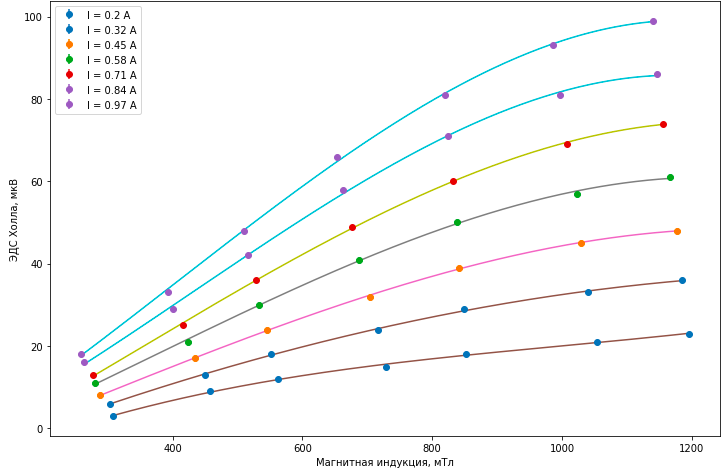
\includegraphics[width=0.9\linewidth]{img/img3.png}
            
            Определение температуры Кюри.
        \end{center}
        \begin{table}[!h]
            \begin{flushleft}%\hspace{80}
           		\textbf{Таблица 3} -- Уравнения полученных прямых: $y = bx + a$.\\
            \end{flushleft}
            \begin{center}
                \begin{tabular}{ | l | l | l | l | l |}
                    \hline
                        &   $b$   &   $a$   &   $\sigma_a$   &   $\sigma_b$ \\
                    \hline
                    Слева, $10^{-3}$   &   2.158   &   -2.431  &   0.205   &   0.412   \\
                    \hline
                    Справа, $10^{-3}$  &   21.04   &   -39.86  &   0.319   &   1.81    \\
                    \hline
                \end{tabular}
            \end{center}
        \end{table}
\newpage
    \subsection{Точка Кюри.}
        Построим графики $(\tau^2 - \tau_0^2) = f(T)$ и $1/(\tau^2 - \tau_0^2) = f(T)$. На втором графике, экстраполируя полученную прямую к оси абсцисс, определим парамагнитную точку Кюри $\Theta_p$ для гадолиния.
        
        Температура Кюри для гадолиния полученная из графика (см. Таблицу 3): 
        \[
        0 = b\cdot T + a, (\text{уравнение } y = bx + a),
        \]
        \[
        0 = 0.0210\cdot T - 0.3987,
        \]
        \[
        T = 18.9 \textdegree C.
        \]
    \subsection{Погрешности.}
        Погрешность вычисления температуры Кюри связана с погрешностью МНК.
        Погрешность прямой, построенной при помощи МНК, записана в таблице 3.
        
        Тогда:
        \[
        \sigma_T = \sqrt{\sigma_b^2 + \sigma_a^2} = \sqrt{0.319^2 + 1.81^2} = 1.83,
        \]
        \[
        \varepsilon = \dfrac{\sigma_T}{T} = 0.096 = 9.6\%.
        \]
\end{document}
